\chapter{Úvod}

Hra Snake patří mezi klasické počítačové hry, které si získaly popularitu díky své jednodu-\\chosti, ale zároveň rostoucí obtížnosti. Tradičně je had ovládán hráčem, avšak v této práci se zaměřím na vytvoření autonomní verze hry, kde had sám dokáže dohrát hru až do zaplnění celého hracího pole. Aby se had mohl efektivně navigovat herním prostředím, bude využívat algoritmy pro hledání nejoptimálnější cesty k jablku a zároveň se vyhýbat kolizím. 

Mezi hlavní metody patří \(A*\) algoritmus, který je široce používán pro hledání nejkratších cest, a algoritmy zaměřené na hledání Hamiltonovských kružnic, které umožňují průchod všemi poli bez opakované návštěvy stejného místa. V práci se budu věnovat nejen implemen-\\taci samotné hry, ale také porovnání různých přístupů z hlediska jejich efektivity, výpočetní náročnosti a schopnosti hada úspěšně dokončit hru.

\section{Hra Snake}

Hra Snake je jednoduchá arkádová hra, ve které hráč ovládá hada pohybujícího se po hracím poli. Cílem hry je sbírat jablka, která se náhodně objevují na hrací ploše. Po sebrání jablka se had vždy prodlouží o jedno políčko. Hra končí v okamžiku, kdy had narazí do stěny nebo do svého vlastního těla.

Hráč ovládá hada pomocí směrových kláves, čímž mění směr jeho pohybu nahoru, dolů, doleva nebo doprava. Had se pohybuje konstantní rychlostí, a jakmile hráč změní směr, had okamžitě reaguje a pokračuje v pohybu daným směrem. Není možné se otočit o 180 stupňů, což znamená, že had nemůže jít zpět po své vlastní trase.

\begin{figure}[H]
    \centering
    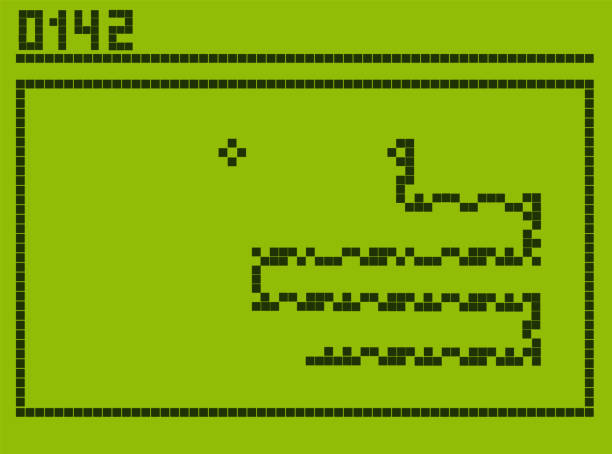
\includegraphics[width=0.5\linewidth]{Images/SnakeGame.jpg}
    \caption[Dostupné z: \url{https://www.istockphoto.com/cs/search/2/image-film?phrase=snake+game}]{Hra Snake}
    \label{fig:SnakeGame}
\end{figure}

V této práci se budu zabývat verzí hry, ve které se had pohybuje v omezeném prostoru s pevnými hranicemi. Hrací pole má obdélníkový tvar a je ohraničeno zdí, která tvoří pevnou bariéru. Jakmile had narazí do této zdi, hra končí. Toto omezení vyžaduje, aby had efektivně plánoval své pohyby a předcházel situacím, kdy by se ocitl v pasti. V této variantě hry neexistuje možnost průchodu skrz okraje obrazovky, což činí navigaci složitější a nutí hada efektivně optimalizovat svůj pohyb.

\section{Zadání práce}
Cílem mé práce je pokusit se o napsání hry Snake, ve které Snake sám dohraje hru (to znamená, že zaplní celý prostor hracího pole, aniž by se zabil). Snake se bude snažit najít optimální cestu k jablku a přitom se bude vyhýbat kolizím. Pomocí různých algoritmů se pokusím o to, aby Snake dokázal najít jablko co nejoptimálněji a pokud možno nejlépe dohrál hru. V práci se budu snažit využít algoritmy na hledání Hamiltonovské kružnice a algoritmus A*. Součástí práce bude porovnání výsledků použitých algoritmů.

\section{Použité technologie}
Práce je napsaná v programovacím jazyce Python, s využitím knihovny Pygame na vykres-\\lování herního pole hry Snake.

\section{Analýza problému a řešení}

Pro úspěšnou implementaci autonomní verze hry Snake je nutné vyřešit několik klíčových problémů. Jedním z hlavních aspektů je reprezentace herního pole a samotného hada. Hrací plocha je modelována jako dvourozměrná mřížka, kde každá buňka může být prázdná, obsahovat tělo hada nebo jablko. Had je reprezentován jako seznam souřadnic jeho těla, kde první prvek odpovídá hlavě hada.

Aby bylo možné efektivně plánovat pohyb hada, problém navigace lze chápat jako hledání cesty v grafu, kde uzly představují jednotlivé buňky hracího pole a hrany odpovídají možným tahům. Hledání nejkratší cesty probíhá mezi hlavou hada a jablkem, což snižuje výpočetní náročnost oproti sledování celého těla. Hlavní výzvou je nejen nalezení efektivní trasy k jablku, ale také zajištění toho, aby had nezablokoval svůj vlastní pohyb a měl dostatečný prostor pro další růst. Kromě toho musí být strategie hada navržena tak, aby umožnila zaplnění celé hrací plochy, tedy úspěšné dokončení hry.